%% *************************************************************************
%%
%% This is an RIT Space Exploration Standard defining guidelines for content
%% and formatting of project design documents.
%%
%% This document uses IEEEtran.cls, the official IEEE LaTeX class
%% for authors of the Institute of Electrical and Electronics Engineers
%% (IEEE) Transactions journals and conferences.
%%
%% *************************************************************************

%% *************************************************************************
% LaTeX REFERENCES
% ----------------
%   Intro to LaTeX: http://www.rpi.edu/dept/arc/docs/latex/latex-intro.pdf
%   Comprehensive LaTeX symbol list: http://tug.ctan.org/info/symbols/comprehensive/symbols-a4.pdf
%% *************************************************************************

% tell \LaTeX what kind of formatting to use
\documentclass[conference]{IEEEtran} % http://www.ctan.org/pkg/ieeetran
% enable placeholder text generator
\usepackage{blindtext}
% enable toolbox for embedding figures and pictures
\usepackage{graphicx}
% enable package for adding a list of variables and constants at the beginning, aka "nomenclature"
\usepackage{nomencl}
% enable package for easily formatting units
\usepackage{siunitx}
% enable package for cross-referencing figures, sections, references etc.
% how to use hyperref: http://www2.washjeff.edu/users/rhigginbottom/latex/resources/lecture09.pdf
\usepackage{hyperref}
% change text encoding to make it more crisp
\usepackage[T1]{fontenc}
% enable conditionals for help text
\usepackage{etoolbox}

\usepackage{float}

\usepackage{array}

%\usepackage{biblatex}
%\addbibreasource{CGT-PDD.bib}

% initialize nomenclature package
\makenomenclature{}

% set title. choose something as descriptive and precise as possible. Descriptive > sounding cool. remember this!
\title{Design \& Implementation of a Cold Gas Thruster}


\author{
  % List the authors of the design document. The Champion should go first.
  % The \$~\$ markers tell \LaTeX{} to treat the text inside to be treated as a math expression. This way you can use operators like \textcaret{} to place characters as superscripts.
  % Some \LaTeX{} templates handle the author block in different ways. For example, the \href{http://www.worldscientific.com/worldscinet/jai}{Journal of Astronomical Instrumentation} requires the authors' addresses and emails to be included as well.
  % The \textbackslash{}thanks command puts the contents inside those brackets in a footnote at the bottom of the first page. Technically speaking, \textbackslash{}thanks is just a specially formatted footnote.
  % IEEE also has a ``long form'' author block for many authors. Check here for more information:
  % \url{https://tex.stackexchange.com/questions/156523/multiple-authors-with-common-affiliations-in-ieeetran-conference-template}
  % Read here for a more advanced options to modifying footnotes in the author block:  \url{http://tex.stackexchange.com/questions/826/symbols-instead-of-numbers-as-footnote-markers}
  %   Here, we use the IEEE long-form author block.
  \IEEEauthorblockN{% This block is for author Names.
    James~Emerson~Parkus\IEEEauthorrefmark{1},  %the number in the bracket is a reference number to identify this footnote. \LaTeX will figure out what symbol to put there.
    David~Breen\IEEEauthorrefmark{2}
  }
  \IEEEauthorblockA{% This block is for the author Afficliations, aka department and university
    RIT Space Exploration, Rochester Institute of Technology \\ %\\ starts a new line
    Rochester, N.Y. \\
    Email:
    \IEEEauthorrefmark{1}jep7631@rit.edu,
    \IEEEauthorrefmark{2}djb1410@rit.edu
}
  %%   Below, we use the short-form author block and basically hack it to suit our needs.
   %James~Emerson~Parkus$^{*\dagger}$%
     %\thanks{$^{*}$Project Champion}%
     %\thanks{$^{\dagger}$BS '20, Mechanical Engineering Technology}

   %David~Breen$^{\ddagger}$%
     %\thanks{$^{\ddagger}$BS '19, Electrical-Mechanical Engineering Technology}

  %%   If there are many authors, consider using symbolic, numeric (aka arabic),  alphabet footnotes or a combination thereof.
  %% the recommended order for symbolic footnotes is
  %%   (1) asterisk        *   *
  %%   (2) dagger          †   \dagger
  %%   (3) double dagger   ‡   \ddagger
  %%   (4) section symbol  §   \S
  %%   et cetera. For higher counts, use 2x symbols (1)-(4) (i.e. (5) two asterisks **). Keep cycling through (1)-(4) using 3x, 4x, and so on.
  %%   Note that these symbol codes work in math mode and text mode.
  %%   There are ways to make LaTeX do this for you, but it is more advanced and not entirely necessary, especially for short author lists. Not worth the hassle, in my opinion.
}
% page header for pages other than cover page
\markboth{Project Design Document Standard}%
{Linden \MakeLowercase{\textit{et al.}}: RIT Space Exploration}

% Initial setup is over, start building the document itself
\begin{document}
\maketitle%
% correct bad hyphenation here, separated by spaces
\hyphenation{explor-ation}

\begin{abstract}
  This project concerns the design, fabrication, and experimentation of a cold gas thruster. The project's main goal is to provide insight
  and experience into the design of a supersonic nozzle for small propulsion systems. Secondary goals will include the understanding
  in the design of high-pressure flow systems, including the necessary precautions and procedures to ensure safe usage. The propulsion subsystem
  will provide the thrust and consist of a high pressure tank, a regulator, a solenoid, and the appropriate piping and interfaces. The structure subsystem will
  will hold the propulsion system in place and allow measurement of the thrust and will consist of aluminum sheet metal and t-slotting. This project will be the first
  step in the design of a cold gas thruster for a CubeSat to allow atmospheric re-entry.
      % The abstract is a brief summary of the design document. Typically it includes the purpose of the design document, key goals or objectives, and justifications.
      % Be sure not to confuse the abstract with the introduction.
      % It is easiest to write the abstract after the rest of the paper has been written.
      % That way you can choose key information from the sections that you've already completed and string them together in the abstract.
      % Consider the abstract to be your elevator pitch to anyone reading this design document.
      % What are they reading?
      % What is the goal?
      % Why is it worth my time?
      % The abstract is what will show up in Google results and other search engines, and what people will read when they are deciding what is worth their time and brain power.
\end{abstract}

\label{sec:nomenclature}
\newcommand{\nomunit}[1]{%
\renewcommand{\nomentryend}{\hspace*{\fill}#1}}
\renewcommand{\nompreamble}{
    % If you include mathematical expressions or express variables in the design document, list them with their corresponding definitions here as a list.
    % The two lines below make it look nice when defining units/values to constants.

    % Note that math terms and non-math terms are separated and alphabetized, regardless of the order in which they are defined. (Recall terms \$like this\$ are in the math environment)
    % Read more about advanced nomenclature formatting here:\\
    % \url{https://www.sharelatex.com/learn/Nomenclatures}
  }
\nomenclature{RIT}{Rochester Institute of Technology}
\nomenclature{SPEX}{RIT Space Exploration}
\nomenclature{CGT}{Cold Gas Thruster}
\nomenclature{RCS}{Reaction Control System}
\nomenclature{$I_{sp}$}{Specific Impulse [s]}
\nomenclature{$I_t$}{Total Impulse [Ns]}
\nomenclature{$g_0$}{Standard gravity [m/s^2]}
\nomenclature{$m_p$}{Propellant Mass [kg]}
\nomenclature{$t_f$}{Final time [s]}
\nomenclature{$t_i$}{Initial time [s]}
%\nomenclature{\gamma}{Specific Heat Ratio}
% Below are examples of using nomenclature for math symbols and constants or units
% \nomenclature{$\dot{m}$}{Mass flow rate
%   \nomunit{\,\si{\kilo\gram\per\second}}}
% \nomenclature{$c$}{Speed of light
%  \nomunit{\,\SI{2.9979e8}{\meter\per\second}}}
\printnomenclature{}


% HELPFUL HINT: If you get the warning ``Command terminated with space.'' when using a \command try placing ``%'' or ``{}'' immediately following the command.

% The sections included here are required. Additional sections and subsections may be added as necessary.
\section{Introduction}
\label{sec:introduction}
  % The introduction is a place to give background and context before diving into the subject matter.
  % Establish context for the work you are about to propose and the main ideas of the proposition itself.

\IEEEPARstart{T}{he} objective of this project is create a cold gas thruster. The CGT will allow the team to gain experience in designing, building,
and testing propulsion systems. The type of nozzle that will be tested is a minimum length supersonic nozzle. There is ambient pressure, thus the
nozzle will be optimized for ambient conditions.

\section{Primary Objective}
\label{sec:primary-obj}
  % At the end of the day, whether the project ``succeeds'' or ``fails'' is judged against the objectives it sought to meet.
  % Note that results that contradict expectations/hypotheses are not failures if the scientific \& engineering methods are followed along the way.
  % Sometimes our expectations are wrong and that can be just as successful as getting data we thought we'd see.
  % What matters are what questions you intend to answer.
  % This is the main purpose or main goal the project hopes to achieve.
The primary objective of this project is to create a cold gas thruster for on-ground experimentation. The goal for the data is to be able to design a nozzle for a small propulsion system, where boundary
layer effects are dominant, but also to achieve an specific impulse of 50s. Using the thrust over time curves, the specific impulse can be
 calculated numerically using MATLAB\@. The data will be transferred and analyzed there using the following equations as a basis.


\begin{equation} \label{specific impulse}
  I_t    = \int_{t_i}^{t_f} F_{thrust} dt
\end{equation}

\begin{figure}[h]
  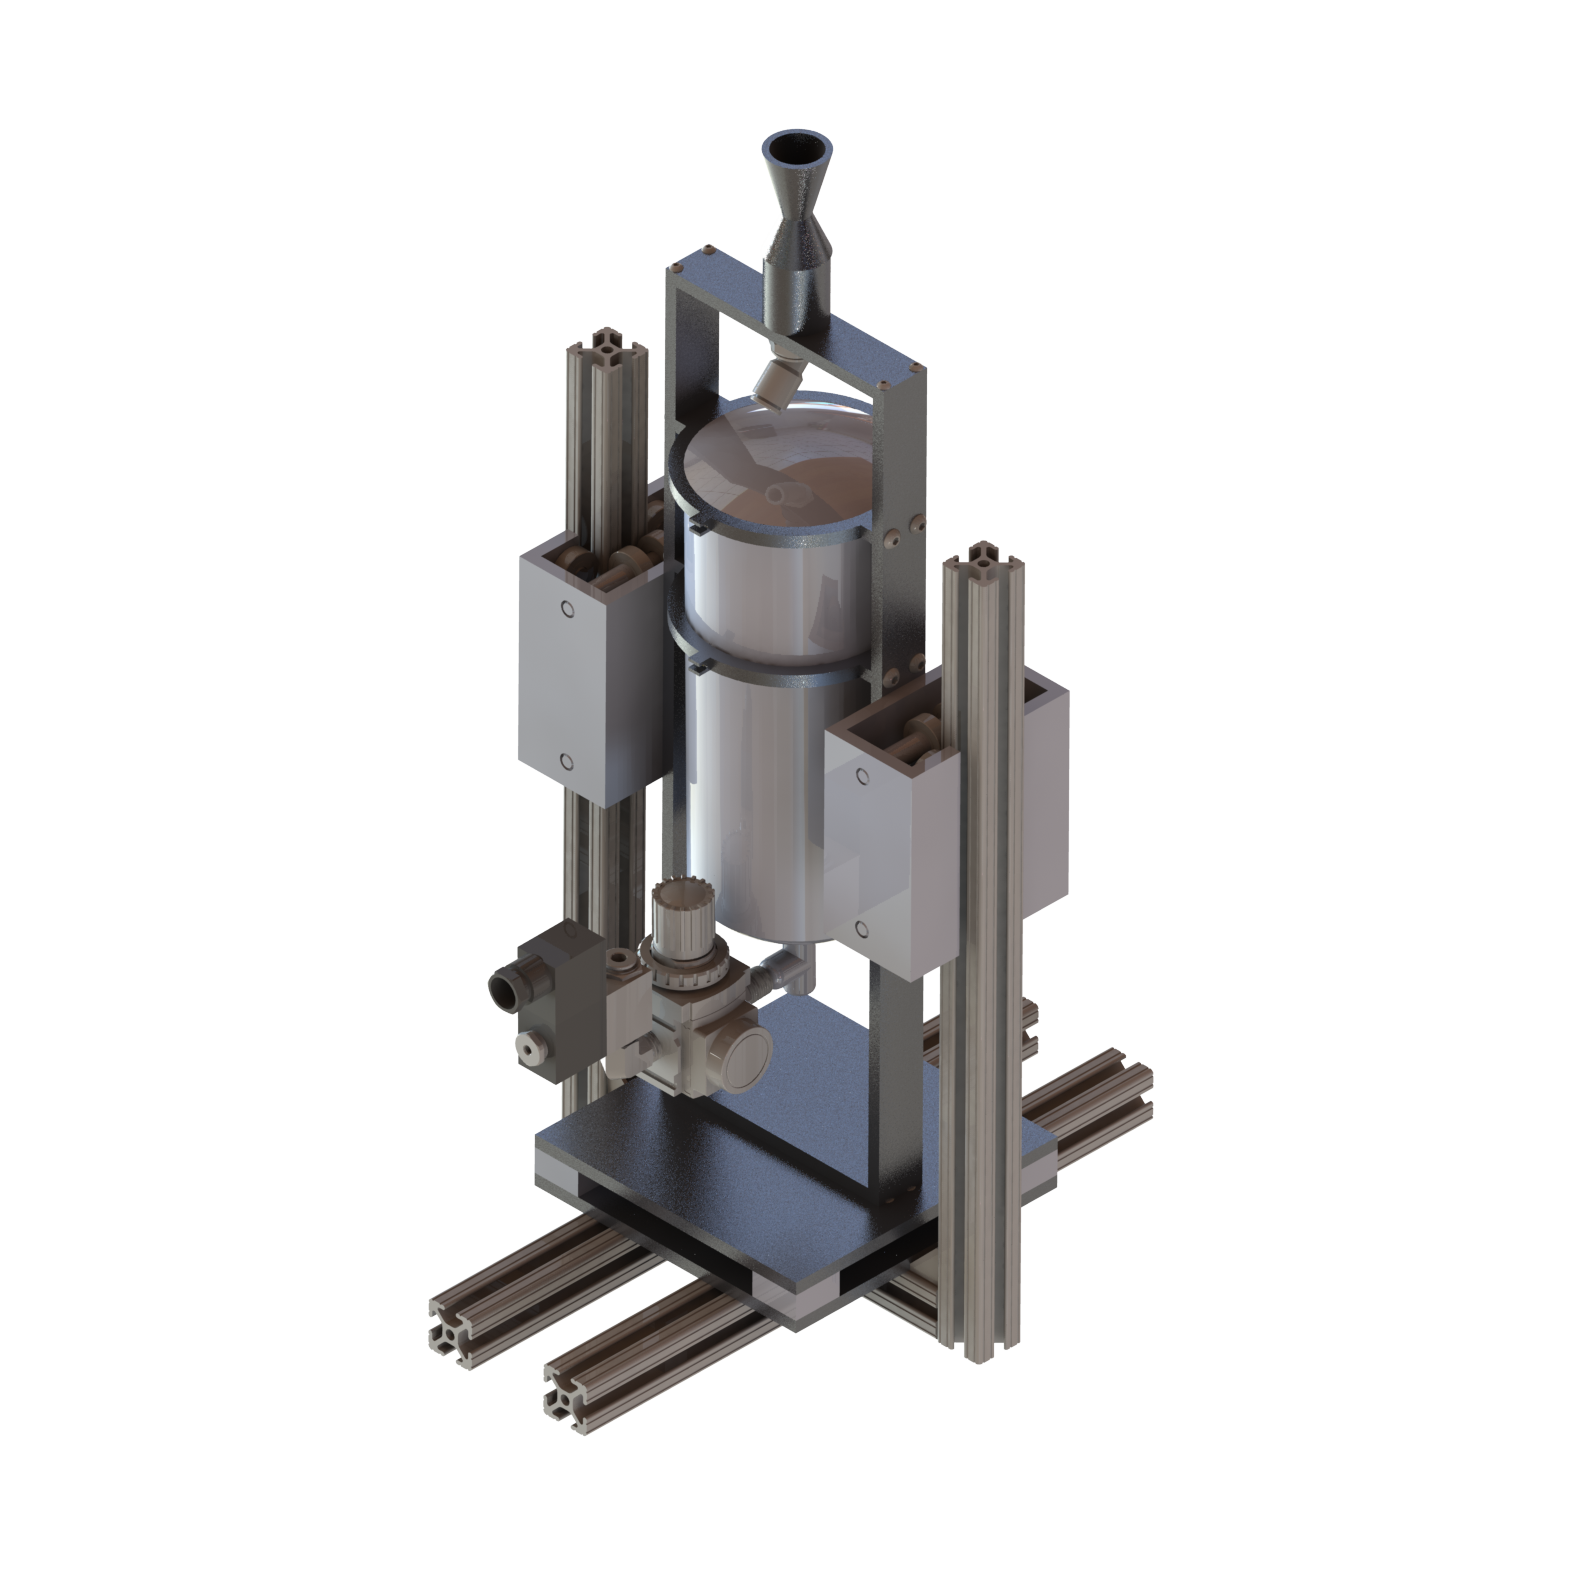
\includegraphics[width=\linewidth]{figs/cold-gas-thruster.png}
  \caption{The Solidworks Assembly of the Spring 2017 design of the SPEX cold gas thruster. The piping from the solenoid to the nozzle is omitted for clarity.}
\label{fig:lifecycle}
\end{figure}

\begin{equation} \label{specific impulse}
  I_s = \frac{I_t}{m_p g_0}
\end{equation}

Data error found from past experimentation was 5\% of the thrust. This error is due to the quality of the load cell. It has an inherent inaccuracy. This
amount of error is acceptable. The performance analysis will not be detrimentally affected. The risk mitigation includes zeroing the load cell just before the test.
This will erase the effects caused by initial weight placed on the load cell. This initial weight comes from the aluminum sliding fixture which holds the nozzle
and the plumbing system.



% \section{Secondary Objectives}
% \label{sec:secondary-obj}
% Secondary Objectives are lower priority or bonus objectives that are significant but not the main focus of the project. This template does not have secondary objectives.

\section{Benefit to SPEX}
\label{sec:benefit}
% One of the core values of SPEX is to provide opportunities for academic and professional growth for its members,
% and to challenge them with interesting projects.
% In this section, explain how the project would benefit SPEX members as students,
% space enthusiasts, and young professionals.

This project can be benefical to SPEX because of the experience given to SPEX in propulsion system design and experimentation. The experience includes learning how to contruct flow systems, design nozzles
for a small propulsion system, and an understanding of the design complexites. These can help avoid roadblocks in future designs. After its completion, SPEX will have a cold gas thruster that
be shown to companies, faculty, students, and at any event where SPEX is on display. The CGT's high mobility will make transportation easy and it is very safe to show to people when the tank is unpressurized. This project
will also be the first foot in the door for CubeSat propulsion. There is also a continuation of this project ready to be initated upon its completion, the
reaction control system.

There are many levels of
analysis that can be used to design one, but the best way is experimentation (trial \& error). This is especially true for cold gas propulsion of this
size. The combination of the size of the nozzle and the high reynolds number of the gas does not allow and analytical solution to the optimal dimensions
of the nozzle. An analytical solution usually concerns making a conical nozzle. However the thrust loss on these nozzles is maxmized. This is due to the
direction of the outgoing flow. The particles travel away from the nozzle at an angle and this increases the horizontal velocity component, and decreases the
vertical velocity (the direction pointing out of the nozzle), which decreases the thrust of the system. Since cold gas propulsion is inherently inefficient, due
to the fact that their is no chemcial reaction or heat applied to the system, maxmizing the thrust is imperitive.

Last, but certainly not least, is the nozzle determination experience. Because of the flow conditions and dimensions, an analytical solution will not be sufficient. To accurately determine
the nozzle size experiementation must happen. This data will be immensely helpful for designing the RCS nozzles and any other CGT nozzles with similar
size magnitudes.

% Below I have used subsections to identify key ideas in this section. These particular subsections are not required as part of the SPEX Standard, but serve as an example of using subsections in a text.

\section{Implementation}
\label{sec:implementation}
  % What path do you anticipate the project to take?

This project will include 4 to 5 weeks of design, 3 to 5 weeks of fabrication, and 4 to 5 weeks of data analysis. The project will start off with a redesign discussion of the test stand, optmizing it for new conditions if necessary.
The team will need to effectively and efficiently determine the appropriate chamber and inlet pressures with varying
nozzle dimensions to create the polynomial curve approximation that will be an integral part of the rest of the research on the topic. Once that is complete, the
testing and experimentation phase begins. At the end of the data analysis the final report will be the main focus. The aim is to complete it by the beginning of winter break
so the team can focus on the new project when they return for the Spring 2018 semester.

\subsection{Deliverables}
\label{subsec:deliverables}
  % When all is said and done, what will you have to show for it?
  % Examples: Hardware, software, poster, ImagineRIT demo, presentations, technical papers...
The deliverables of this project will be split into to two sections, physical and non-phsyical.

\subsubsection{Physical Deliverables}
\label{subsubsec: physical deliverables}

The propulsion system will include a regulator, a solenoid, a tank, a nozzle, piping, and the interfaces all connected in a series.
The test stand will include the t-slot frame with the tank frame. They will be made entirely of aluminum. Aluminum is a great material for its balance of strength, machinability, and
weight. Steel is very difficult and hardous to machine and is very heavy, although its strength is greater than aluminum. Plastics are tedious to machine as they tend to melt to the cutting
blade and that casues the machining to stop frequently to clean off the blade. The propulsion has a very large pressure drop and this will cause a large temperature drop. A plastic structure will
effected greatly by this and will harden to the point where fracture could occur very easily. The interfaces between the
aluminum parts will also be included. This consists of the various t-slot connections and the bolts and washers that connect the aluminum sheets.

There will also be an arduino connected to a computer that will use Simulink for data acquisition. The arduino will be a conduit to relay the data from the load cell
to Simulink. There will also be an arduino to control the use of the solenoid. The solenoid will be activated from the Simulink program, which will coincide with
the beginning of data acquisition.

The system will also be displayed at Imagine RIT 2018. This will include a full poster and data representation.

\subsubsection{Non-physical Deliverables}
\label{subsubsec: non-physical deliverables}

The non-physical deliverables of this project will be the project culmination report which will include a very detailed examination of the projects
results. These results include the expected performance versus the test performance, the nozzle dimension polynomial approximation, the structure performance, and the
propulsion system performance. The structural performance is a section that discusses the reasoning behind the initial design and any problems
that were found during testing. The problems to be avoided will be, unecessary frictional loss due to bad connection points or instability of the test stand due to
bad interfacing between structural components. The propulsion system performance will be very similar to this except it will focus on slightly different aspects, such as
the mass flow under various ambient conditions and temperatures. The propulsion performance will mostly be measured through the data analysis. This specifically concerns the
specific impulse. It will also concern the expansion of the flow, as the maximum thrust will occur when the exit pressure equals the ambient pressure and thus the shocks
in the flow will expand optimally. This will be observed through schlieren lensing, as it has been performed before during nozzle testing. This was performed in the Spring 2017
semester for flow visualization. The procedure was; turn the lights off, put the nozzle on the air hose, put a white piece of paper on a table, put it parallel to the table, initiate the cold burn, use a phone light
to project the flow onto the white paper below it. Then distance between the nozzle and the light and the table were toggled until the best focus point was found. That is how the team
was able to get the picture below.

\begin{figure}[h]
  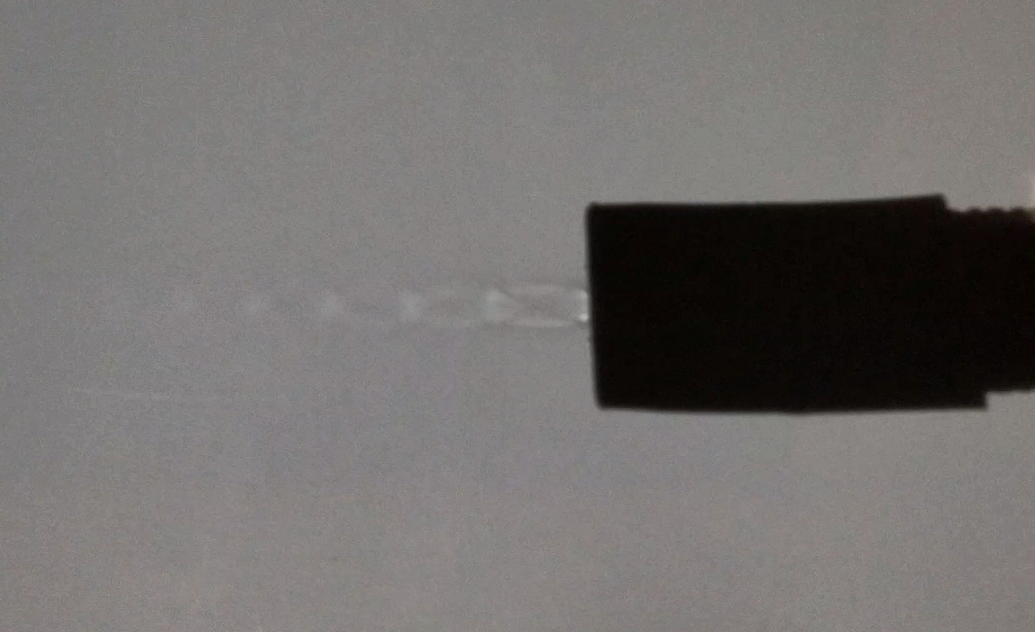
\includegraphics[width=\linewidth]{figs/nozzle-shocks[2].png}
  \caption{The flow is seen here exiting a small 3D printed supersonic nozzle. The procedure was not unlike schlieren lensing, but the clarity was much lower.}
  \label{fig: nozzle shocks}
\end{figure}

\subsection{Milestones}
\label{subsec:milestones}
  % Be as detailed as you can, but it's okay if there are unknowns.
  % At the very least, specify how many semester you expect the project to take until it reaches completion.

There is a preliminary plan for the semester that is displayed in further detail in Appendix A. The following list will display the description and timing
of the different phases; design, sanity tests, experimentation, and data analysis.

\subsubsection{Design Phase}
\label{subsubsec: design phase}
    The goals are to design the propulsion system, the test stand, the nozzle. At the end of this phase
    there will be a full system CAD model and a series of CAD nozzles to be fabricated. This CAD model is essential for the next phase, as the fabrication
    will use it as a guide (inlcuding drawings for machinists).

    \textit{Projected Duration: 2-3 weeks}

\subsubsection{Build \& Preliminary Test Phase}
\label{subsubsec: sanity test phase}
    This phase is concerned with the building of the system. The test stand is already built. However if minor revisions are necessary, then the team will
    build the new design (any re-design will concern the dimensions of the tank fixture and will therefore not take long as it is a simplistic system).
    The main part of the building stage will be the construction of the propulsion system. That is where most of the work will be. Once the system is built,
    it will be tested at component-level then tested at system-level. This is to ensure there are no catastrophic problems during the experiment.
    There will be no data collected during this phase.

    \textit{Projected Duration: 3-5 weeks}

\subsubsection{Experimentation}
\label{subsubsec:experimentation}
    This phase is primarily concerned with the testing of the CGT\@. This includes gathering all the necessary data and experience to create the
    polynomial approximation and to aid in the RCS phase and CREST phase of space propulsion research.
    The testing will consist of 5 tests for each different chamber pressure. These chamber pressures will be; 80, 90, 100, 120, 140, 160, 180, and 200 Psi. There
    will be a total of 40 tests, if time permits there can be more but this is the goal as it will serve as sufficient data for data analysis.
     The data will be averaged for each chamber pressure and then plotted against the nozzle area ratio. Then a tenth-order polynomial
    will be fit to the curve and used to determine a first-order approximation of the nozzle area ratio for future cold gas propulsion systems.

    \textit{Projected Duration: 2-3 weeks}

\subsubsection{Data Analysis}
\label{subsubsec: data analysis}
    This phase is concerned with the analysis of the data collected from the CGT testing. The polynomial approximation will be completed during this
    phase for the minimum length nozzle. It is also the phase where the performance analysis takes place. This will inlcude the ultimate calculation of the specific impulse
    of the thuster and if it attains the values we need to achieve the necessary velocity change for orbital decay to initiate atmospheric reentry.

    \textit{Projected Duration: 3 weeks}

\subsubsection{Final Report}
\label{subsubsec: final report}
    At the end of this project a final report will be made to report the outcome. It will outline the design process, fabrication process, and testing process.
    It will also include the nozzle theory used in the calculations along with all the relevant assumptions and exterior information as needed. The report will provide
    all the test data and data analysis results. The final product for the report will be the discussion of the polynomial curve-fit. This will be an extremely useful tool
    for future similar cold gas propulsion systems and must be discussed in depth with an example of how it will be used.

    Once this paper is complete it will be given to the advisors of the SPEX research group for review and then further publications will be discussed. The paper would
    be great for job interviews to display the work you have done in a formal manner, and one that the interviewer can refer back to at a later date.

    \textit{Projected Duration: 2 weeks}

\section{Externalities}
  % Things not directly related to the work or outcomes, but related to the project as a whole.
\subsection{Prerequisite Skills}
  % Which skills do team members need to have before work can start (not including skills that will be learned ``on the job'')?

Creating a CGT will require a few skills, many of which can be learned throughout the project. The design process will require knowledge of systems and how they
work together, basic nozzle theory, computer-aided design (CAD), basic electrical engineering, basic coding abilities, and machining. The majors that would
be most qualified for satisifing these requirements are mechanical engineering \& technology and electrical engineering \& technology. But this project is certainly
open to all majors because most of these skills can be taught in at least a basic manner.

The basic nozzle theory required here can be adequately learned by reading the introductory chapters of "Rocket Propulsion Elements" by Sutton. Chapter 1 through 4 will
provide a sufficient basis of understanding for this project.

 The CAD software of choice is Solidworks. It is very common for industry and has all the features that the team
will need throughout the process. The education edition also includes the simulation premium package that can allow the team to run flow simulations if needed. The procedure for
doing this is complicated but can be learned to a basic degree on youtube.

The basic electrical engineering including setting up and arduino or raspberry pi to read out the data from the load cell and turning the solenoid on and off. It
should not be difficult for a first year or second year EE or EET to set this up. If it proves to be difficult, the team can each out to older students or professors for assistance.
Dr. Patru would certainly be a great resource for this kind of help.

The basic coding abilites include writing a MATLAB script to analyze and plot data. MATLAB is easy to learn and is very powerful. It is a very common choice for data analysis for mechancial engineering
projects where the core skill set is not computer science. This is not hard for anyone who has coded before.

The machining will be the most difficult to learn if there are no MEs or METs that have taken the proper courses. Machining can be extremely dangerous and cannot be done
without the proper safety training. If no one is trained on the machines one can ask a machinist to make simple parts or submit a job at the Earl Brickman Machine Tools and Manufacturing Lab.
They have professional engineers there that can make nearly anything one could need. But their timeline slips often, so leave an appropriate amount of time for them to make the part
so it does not interfere with the projects timeline.

\subsection{Funding Requirements}
  % Estimate costs that would be needed to meet objectives.
Fortunately, most of the materials for the test stand have been purchased. This eliminates much of the system cost. The most costly part of the project
will be the propulsion system (the regulator, solenoid, nozzle, piping, and interfaces). A preliminary budget that includes margin for cost overruns is \$600.
The total cost was approximately \$450. That would be the last part of the system needed before testing can occur. Accounting for unforseen cost then rounding upwards,
the consquentical estimated cost is put at \$600 for the entirty of the project. A bill of materials is displayed in Appendix B. The table, displayed below, outlines
the most expensive parts that the team will need to purchase for the propulsion system, these parts are worst-case scenario in cost and measures will be taken to
try to alleviate these costs.

\centering
\begin{tabular}{ |p{2cm}|p{2cm}|p{2cm}| }
  \hline
  \multicolumn{3}{|c|}{Propulsion Part List} \\
  \hline
  Part & Cost & McMaster Part \# \\
  \hline
  Tank & \$ 131.35 & 7822A11 \\
  \hline
  Regulator & \$ 182.50 & 49305K21 \\
  \hline
  Solenoid & \$ 100.49 & 4711K511 \\
  \hline
\end{tabular}


\subsection{Faculty Support}
  % Identify faculty that will be involved (or would need to be involved) to meet objectives.
  % Note that if a professor is the Principal Investigator (P.I.) for a project, there still needs to be a student as the SPEX Project Champion.
Little faculty support will be necessary. The SPEX propulsion team has consulted faculty about structure and flow system concerns and made the suggested changes. Most of the
faculty support was needed during the endevour to fabricate the structure and design the flow system.
This included the flow system and how it operates. Dr.Garrick, MET department head, assisted the team in the design of the flow system and pointed out unnecessary components, such
as the flow straightener. He said that the flow was at such a high reynolds number that straightening it in the size constraints is impossible with our budget.
There may be some assistance required if the nozzle performance is far below nominal, but guessing from past work it will not be a problem. This would concern the nozzle design.
Nozzle design is very difficult for the necessary size for the CGT, about 1 inch in length and 0.5 inches in diameter. Boundary layer effects are dominent. To accurately design them
on a computer would include high level numerical smulation which beyond the team's skill set. If there are recurring problems here, Dr. Olles can be consulted as he has experience with this.
There may also be the need for assistance during the data analysis phase or if the team chooses to perform flow simulations. But it will be a small amount of help.

If assistance is needed for the data analysis, Dr. Olles would be a good professor to ask. He has a PhD in rocket science
so he could certainly help.
\subsection{Long-Term Vision}
\label{sec:vision}

The long term vision of this project is to be a building block to the next phase of space propulsion research. CREST, a mission that was proposed in the
spring of 2016 by James Parkus, relies on a space propulsion system. It is the reason the SPEX propulsion subsystem was formed. Thus, it is natural for the
CGT to assist in the furthering of this project. The main conern for CREST was the propulsion necessary to de-orbit quickly enough that SPEX can determine its entry location and therefore estimate its landing location.

This project will also be great for
the members to put on their resume. At the end of this project a detailed document will be made which outlines the most important aspects of the project.
Then the RCS will build off the momentum created by this project. And the understanding of space propulsion inside SPEX will continue to grow and flourish.

Once the CGT is complete, the team can move onto the next phase of space propulsion research. This is the RCS\@. Reaction control systems are used very
frequently in space propulsion and attitude adjustment systems as well as rockets. Building an RCS is difficult. But if the team
has prior experience with cold gas propulsion, their job becomes significantly easier. The team can refer back to their data for the determination of the
appropriate nozzle characteristics.

After the culmination of the cold gas thruster project, the team can try to design, fabricate, and test an aerospike nozzle, only if time permits.
There are benefits to aerospikes but there are also disadvantages. The advantages are concerned with the region of optimal expansion. The aerospike nozzle can match the
ambient pressure over a larger region and therefore can produce more thrust. However, the disadvantages are increased thermal loading and high design and fabrication complexity.

\section*{Acknowledgements}
The author would like to thank Dr. Garrick and Dr. Olles for their help in understanding the theory of nozzles and the review of the system before testing.


\onecolumn
\appendices{}
\section{\textbf{Detailed Fall Timeline}}
\centering
\begin{tabular}{ |p{1.25cm}||p{11.0cm}| }
  \hline
  Week \# & Plan \\
  \hline
  1 & Introductions \& Fall plan discussion \\
  \hline
  2 & Beginner Project: Supersonic Nozzle Design  \\
  & Design Phase: Test stand \\
  \hline
  3 & Beginner Project: Nozzle Printing and Testing on weekend \\
  & Design Phase: Propulsion System \\
  \hline
  4 & Design Phase: Propulsion System \\
  \hline
  5 & Design Phase: Arduino and MATLAB design \\
  \hline
  6 & Design Phase: Arduino and MATLAB design \\
  \hline
  7 & Fabrication Phase: Material order and making Solidworks drawings\\
  \hline
  8 & Fabrication Phase: Machining \\
  \hline
  9 & Fabrication Phase: Machining and assembly \\
  \hline
  10 & Experimentation Phase: Test 1 \\
  \hline
  11 & Experimentation Phase: Test 2 \\
  \hline
  12 & Data Analysis Phase: Data Organization \\
  \hline
  13 & Data Analysis Phase: Noise and error analysis \\
  \hline
  14 & Data Analysis Phase: Performance Analysis \\
  \hline
  15 & Project Culmination Report writing \\
  \hline
  16 & Project Culmination Report finalization \\
  \hline
\end{tabular}

\newpage
\section{\textbf{Cold Gas Thruster Preliminary Bill of Materials}}

\centering
\begin{tabular}{ |p{4cm}||p{1.0cm}|p{1.5cm}|p{2.5cm}|p{2.0cm}|p{2.0cm}| }
  %\hline
  %\multicolumn{6}{|c|}{Cold Gas Thruster Bill of Materials} \\
  \hline
  Part & Cost & Quantity & Vendor & Part Number & Status \\
  \hline
  Tank & \$131.35 & 1 & McMaster Carr & 7822A11 & Not acquired \\
  \hline
  Regulator & \$182.50 & 1 & McMaster Carr & 49305K21 & Not acquired \\
  \hline
  Solenoid & \$100.49 & 1 & McMaster Carr & 4711K511 & Not acquired \\
  \hline
  Push-to-connect fitting & \$4.33 & 2 & McMaster Carr & 5779K116 & Not acquired \\
  \hline
  Aluminum Pipe & \$2.45 & 2 & McMaster Carr & 50785K172 & Not acquired \\
  \hline
  Nylon Pipe & \$8.90 & 1 & McMaster Carr & 5548K77 & Not acquired \\
  \hline
  Aluminum Sheet & \$7.00 & 1 & McMaster Carr & 8975K596 & Acquired \\
  \hline
  Aluminum T-Slot & \$6.49 & 7 & McMaster Carr & 47065T101 & Acquired \\
  \hline
  T-Slot Corner Frame & \$7.98 & 10 & McMaster Carr & 5537T51 & Acquired \\
  \hline
  T-Slot Length Frame & \$5.66 & 4 & McMaster Carr & 47065T235 & Acquired \\
  \hline
  \#8 Socket Head Cap Screws & \$6.58 & 1 [100] & McMaster Carr & 92196A194 & Acquired \\
  \hline
  Arduino & \$10.00 & 1 & RIT Construct & Unknown & Not Acquired \\
  \hline
  Grand Total & \$608.25 & N/A & N/A & N/A & N/A \\
  \hline
\end{tabular}

\bibliography{CGT-PDD.bib}
\printbibliography

\end{document}
